Our dataset consists of 6 seasons of ``play-by-play'' soccer games from major professional leagues such as Li Liga (Spain), English Premier League (EPL), and Major League Soccer (MLS). For a given game between two teams, ``play-by-play'' data identifies each player, their x and y coordinates in the field, a timestamp of hour, minute, and second, and the major action taken by that player, such as a pass, interception, aerial shot, goal etc. in a standardized vocabulary. 

We collected the annotated data from OPTA, a sports analytics company, which ensured data fidelity and annotated player actions (passing, aerial shots) using uniform video annotation techniques. Overall, the dataset consists of 2,280 games from  players across 60 diverse teams, leading to  3,893,304 player actions (rows). Since only one player is considered in each timestep, we can identify player A passed to player B by considering the action and players in successive timestamps.  

\subsection{EPL Dataset}
To prototype our methods, we have only tested our analysis on the EPL dataset.
For the final project, we will repeat the analysis for all leagues, cluster playing styles across leagues, and compare node feature vectors between leagues.

The EPL dataset consists of a single season in 2012, consisting of 380 matches between 20 teams, such as Liverpool, Manchester United, Southampton, etc. The dataset consists of 648,883 unique plays made by 524 unique players, who are annotated to have 5 positions of Strikers, Defenders, Midfielders, Goalkeepers, and Substitutes. Each play is annotated using a standardized vocabulary of 46 actions, including `Goals' and `Interceptions'.


\subsection{Graph Structure}
The team structure within a given match is represented as a weighted, directed graph, where nodes are players and edges are actions (pass, kick, etc.). Our initial networks also include additional event nodes to represent non-player states such as the gaining of the ball, the loss of a possession, and a shot taken. Respectively these are named ``Gain'', ``Loss'', ``Shot'', and ``Goal''. 

\tu{Nodes:}  14 to 17 nodes consist of 11 players from each team plus events and substitute players. As of now we encode no additional information on the nodes except for ID, but will eventually add in position, location, and time played. 

\tu{Edges:} Actions between states where the ball is located. If player (node) A passed to player (node B) some amount of times within a game, a passing edge is created. Concurrently, shot, gain, and loss rates are also used to connect player nodes to event nodes. The weights on the edges can be formulated as follows: 

\begin{enumerate}

    \item Passes (A, B) = (num. successful passes between A and B) / (time shared between A and B)

    \item Shots(A) = (num. saved attempts, post hits, misses, or goals) / (time A on field) 

    \item Gain(A) = (num. of ball recoveries, corners awarded, out of bounds rewarded) / (time A on field) 

    \item Loss(A) = (num. unsuccessful passes, out of bounds, dispossessions) / (time A on field) 

\end{enumerate}


\begin{figure}[h]
  \centering
  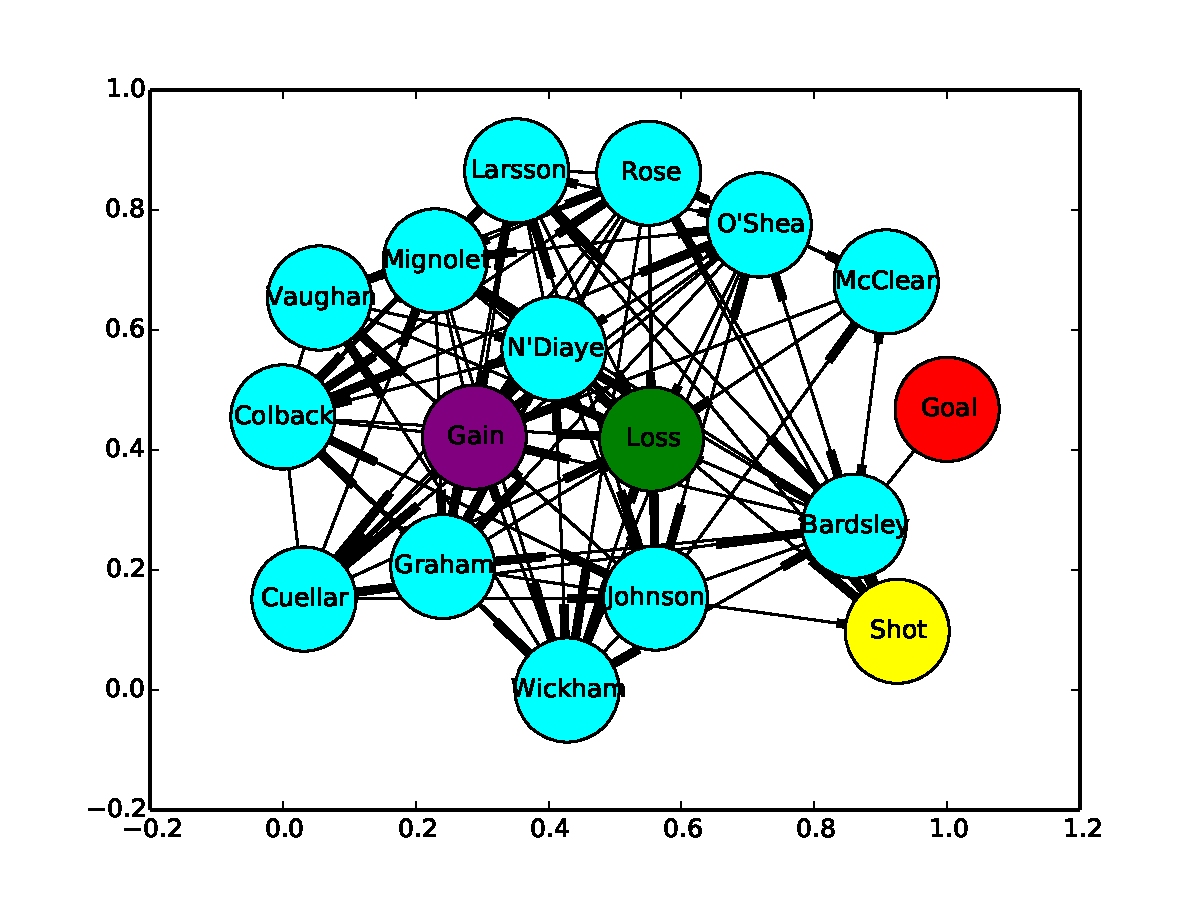
\includegraphics[width=0.45\textwidth]{plots/soccer_networkx.pdf}
  \caption{Example Graph Structure for a Single Team in a Single Game. Player nodes are colored in cyan and edge weights (passing rates) are omitted for visual clarity.}
\end{figure}


\begin{figure}[h]
  \centering
  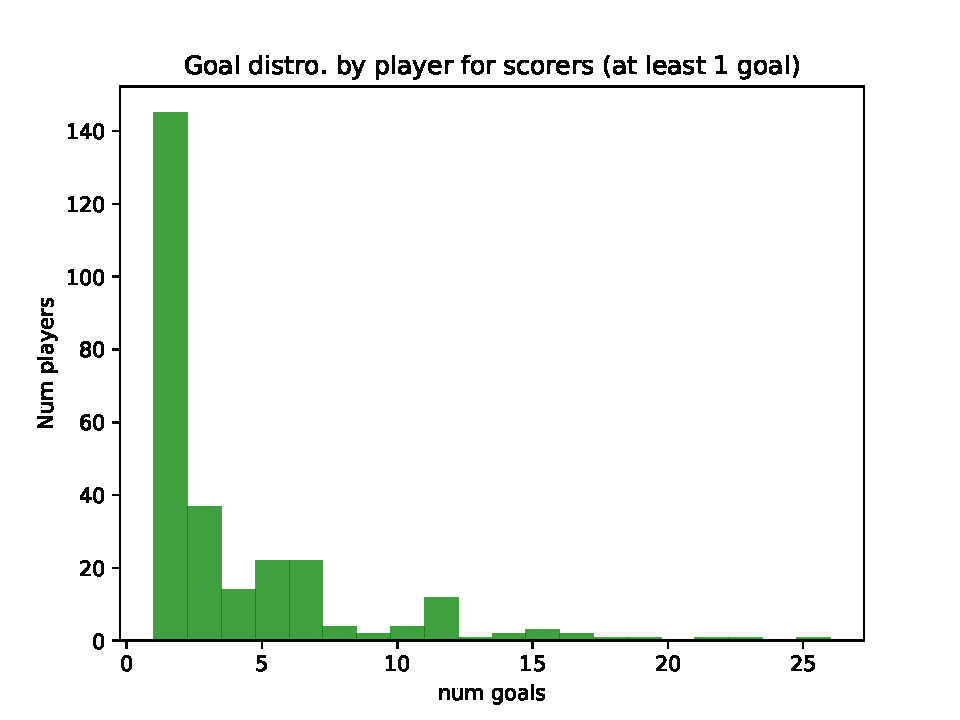
\includegraphics[width=0.45\textwidth]{plots/eplper_player_goal_hist.pdf}
  \caption{Per-player goal distribution across a season.}
\end{figure}



Networks currently in production represent a single team in a single game, such as:

\begin{enumerate}
    \item Single game networks with 2 teams. Each team is connected through respective losses and gains of possessions, transforming original ``Gain'' and ``Loss'' nodes into ``Switch'' nodes.

    \item Aggregated team network consisting of data within a whole season. Each team's individual networks is aggregated across all games, giving one unique network per team. Rates are now based on total time rather time in a game. 
\end{enumerate}

\subsection{Data Processing}

Our initial code processes the play-by-play using 2 pointers that track players making actions, and players receiving actions. Time on field is measured through substitution events, where in the event a substitution doesn’t occur, the player is assumed to have played the whole game. These counts of actions are stored in a dictionary representing an edge list where keys are tuples of player IDs. The time metrics are then used to transform these dictionary components into rates. Additional information tracked include team, home vs away status, goals, winning team, and match id. 

As a sanity check, we plotted the distribution of goals across a season for EPL players that scored at least once. Figure 2 shows a reasonable distribution between 1 goal (the mode) and a maximum of 26 per-player season goals. The edge list dictionary is used to create a passing-rate weighted TNEANet graph in snap. 




